\documentclass[titlepage,landscape]{seminar}
\usepackage{url}
\usepackage{graphicx}
\usepackage[pdftex]{color}
\usepackage{hyperref}
\usepackage{epstopdf}
\usepackage{slides}

\begin{document}

\myslide{
\begin{eqnarray*}
q_{t+\Delta t} &=& (1 - \lambda\Delta t)^2q_t
                  + 2\left(1 - \lambda\Delta t\right)\left({1 \over
                           3}\lambda\Delta t\right)(1 - q_t)
                  + \hbox{o}(\Delta t^2) \\
               &=& (1 - 2\lambda\Delta t)q_t + \left({2 \over 3}\lambda
                                                    \Delta t\right)
                                              (1 - q_t) 
                  + \hbox{o}(\Delta t^2)
\end{eqnarray*}
\begin{eqnarray*}
q_{t+\Delta t} - q_t &=& {2 \over 3}\lambda\Delta t - {8 \over
                           3}\lambda\Delta tq_t + \hbox{o}(\Delta t^2) \\
{q_{t+\Delta t} - q_t \over \Delta t} &=& {2 \over 3}\lambda - {8 \over
3}\lambda q_t + \hbox{o}(\Delta t) \\
\lim_{\Delta t\to 0}{q_{t+\Delta t} - q_t \over \Delta t}  = {dq_t \over dt} &=& {2 \over 3}\lambda - {8
\over 3}\lambda q_t \\
q_t &=& 1 - {3 \over 4}\left(1 - e^{-8\lambda t/3}\right) \\
\end{eqnarray*}
}

\myslide{
Number of substitutions: $d = 2\lambda t$
\vfil
\begin{eqnarray*}
q_t &=& 1 - {3 \over 4}\left(1 - e^{-8t/3}\right) \\
    &=& 1 - {3 \over 4}\left(1 - e^{-4d/3}\right) \\
d   &=& -{3 \over 4}\ln\left[1 - {4 \over 3}(1 - q_t)\right] 
\end{eqnarray*}
}

\myslide{
From Britten {\it PNAS\/} 99:13633-13635; 2002.

\begin{itemize}

\item 5 Chimpanzee genome sequences totaling 779,142bp

\item Aligned with ``the'' human genome

\item 1.41\% nucelotide sequence difference~(additional 3.91\%
  difference in idels)

\end{itemize}

\begin{eqnarray*}
d &=& -{3 \over 4}\ln\left(1 - {4 \over 3}(0.0141)\right) \\
  &=& -{3 \over 4}\ln(0.9812) \\
  &=& 0.0142
\end{eqnarray*}

For ``small'' amounts of sequence divergence $d \approx 1-q_t$.
}

\myslide{
From Liu et al. {\it Genome Research\/} 13:358-368; 2003.

\begin{itemize}

\item 623,139 aligned nucleotides between humans and lemur

\item 19.4\% nucleotide sequence difference

\end{itemize}

\begin{eqnarray*}
d &=& -{3 \over 4}\ln\left(1 - {4 \over 3}(0.194)\right) \\
  &=& -{3 \over 4}\ln(0.7413) \\
  &=& 0.22
\end{eqnarray*}

For ``large'' amounts of sequence divergence the number of
substitutions distinguishing two sequences is much larger than the
observed number of differences.
}

\myslide{
Suppose two sequences have been diverging for a very, very long time.

Then the probability that they match at any given nucleotide will be
about 1/4.

\begin{eqnarray*}
d &=& -{3 \over 4}\ln\left(1 - \left({4 \over 3}\right)\left(1- {1
      \over 4}\right)\right) \\
  &=& -{3 \over 4}\ln\left(1 - \left({4 \over 3}\right)\left({3 \over
        4}\right)\right) \\
  &=& -{3 \over 4}\ln(0) \\
  &=& \infty
\end{eqnarray*}
}

\myslide{
\begin{eqnarray*}
\mbox{\# of substitutions/generation} &=& (\mbox{\# of
  mutations/generation}) \\
                                      && \times(\mbox{probability
  of fixation}) \\
\lambda &=& \mu_0p_0 
\end{eqnarray*}
\vfill
\[
\mu_0 = 2N\mu
\]
\vfil
\[
p_0 = \frac{1}{2N}
\]
\vfill
\[
\lambda = 2N\mu\left(\frac{1}{2N}\right) = \mu 
\]
}

\myslide{
\[
f = \frac{1}{4N_e\mu + 1}
\]
\vfill
\[
H = \frac{4N_e}{4N_e\mu + 1}
\]
\vfill
}

\myslide{\tiny
\begin{center}
\begin{tabular}{llllllll}
\hline\hline
      & Amino &       & Amino &       & Amino &       & Amino \\
Codon & Acid  & Codon & Acid  & Codon & Acid  & Codon & Acid \\
\hline
UUU   & Phe   & UCU   & Ser   & UAU   & Tyr   & UGU   & Cys \\
UUC   & Phe   & UCC   & Ser   & UAC   & Tyr   & UGC   & Cys \\
UUA   & Leu   & UCA   & Ser   & UAA   & Stop  & UGA   & Stop \\
UUG   & Leu   & UCG   & Ser   & UAG   & Stop  & UGG   & Trp \\
      &       &       &       &       &       &       & \\
CUU   & Leu   & CCU   & Pro   & CAU   & His   & CGU   & Arg \\
CUC   & Leu   & CCC   & Pro   & CAC   & His   & CGC   & Arg \\
CUA   & Leu   & CCA   & Pro   & CAA   & Gln   & CGA   & Arg \\
CUG   & Leu   & CCG   & Pro   & CAG   & Gln   & CGG   & Arg \\
      &       &       &       &       &       &       & \\
AUU   & Ile   & ACU   & Thr   & AAU   & Asn   & AGU   & Ser \\
AUC   & Ile   & ACC   & Thr   & AAC   & Asn   & AGC   & Ser \\
AUA   & Ile   & ACA   & Thr   & AAA   & Lys   & AGA   & Arg \\
AUG   & Met   & ACG   & Thr   & AAG   & Lys   & AGG   & Arg \\
      &       &       &       &       &       &       & \\
GUU   & Val   & GCU   & Ala   & GAU   & Asp   & GGU   & Gly \\
GUC   & Val   & GCC   & Ala   & GAC   & Asp   & GGC   & Gly \\
GUA   & Val   & GCA   & Ala   & GAA   & Glu   & GGA   & Gly \\
GUG   & Val   & GCG   & Ala   & GAG   & Glu   & GGG   & Gly \\
\hline
\end{tabular}
\end{center}
}

\myslide{
\begin{center}
\begin{tabular}{lll}
\hline\hline
      & Amino & \\
Codon & Acid  & Redundancy \\
\hline
CCU   & Pro   & 4-fold \\
CCC \\
CCA \\
CCG \\
\hline
AAU   & Asn   & 2-fold \\
AAC \\
AAA   & Lys   & 2-fold \\
AAG \\
\hline
\end{tabular}
\end{center}
}

\myslide{\scriptsize
\begin{center}
\begin{tabular}{lcc}
\hline\hline
Locus     & Non-synonymous rate & Synonymous rate \\
\hline
Histone \\
\quad H4  & 0.00                & 3.94 \\
\quad H2  & 0.00                & 4.52 \\ 
Ribosomal proteins \\
\quad S17 & 0.06                & 2.69 \\
\quad S14 & 0.02                & 2.16 \\
Hemoglobins \& myoglobin \\
\quad $\alpha$-globin & 0.56    & 4.38 \\
\quad $\beta$-globin  & 0.78    & 2.58 \\
\quad Myoglobin       & 0.57    & 4.10 \\
Interferons \\
\quad $\gamma$  & 3.06          & 5.50 \\
\quad $\alpha$1 & 1.47          & 3.24 \\
\quad $\beta$1  & 2.38          & 5.33 \\
\hline
\end{tabular}
\end{center}
}

\myslide{
\begin{table}
\begin{center}
\begin{tabular}{l|ccc}
\hline\hline
         & 5' flanking & {\it Adh\/} locus & 3' flanking \\
\hline
Diversity$^1$ \\
\quad Observed & 9     & {\bf 14}   & 2    \\
\quad Expected & 10.8  & 10.8 & 3.4  \\
Divergence$^2$ \\
\quad Observed & 86    & 48   & 31   \\
\quad Expected & 55    & {\bf 76.9} & 33.1 \\
\hline
\multicolumn{4}{l}{\footnotesize $^1$Number of polymorphic sites within {\it
         D. melanogaster\/}} \\
\multicolumn{4}{l}{\footnotesize $^2$Number of nucleotide differences between {\it
         D. melanogaster\/} and {\it D. simulans}}
\end{tabular}
\end{center}
\caption{Diversity and divergence in the {\it Adh\/} region of {\it
    Drosophila}~(from Kreitman and Aguade 1986).}
\end{table}
}

\myslide{
\begin{center}
\resizebox{0.8\textwidth}{!}{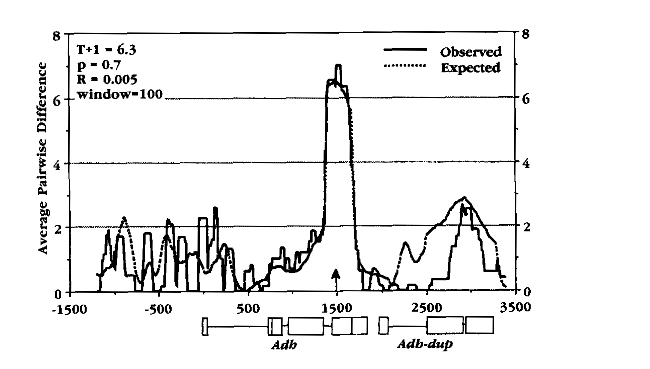
\includegraphics{kreitman-hudson.eps}}
\end{center}
}

\myslide{
\begin{center}
\resizebox{0.9\textwidth}{!}{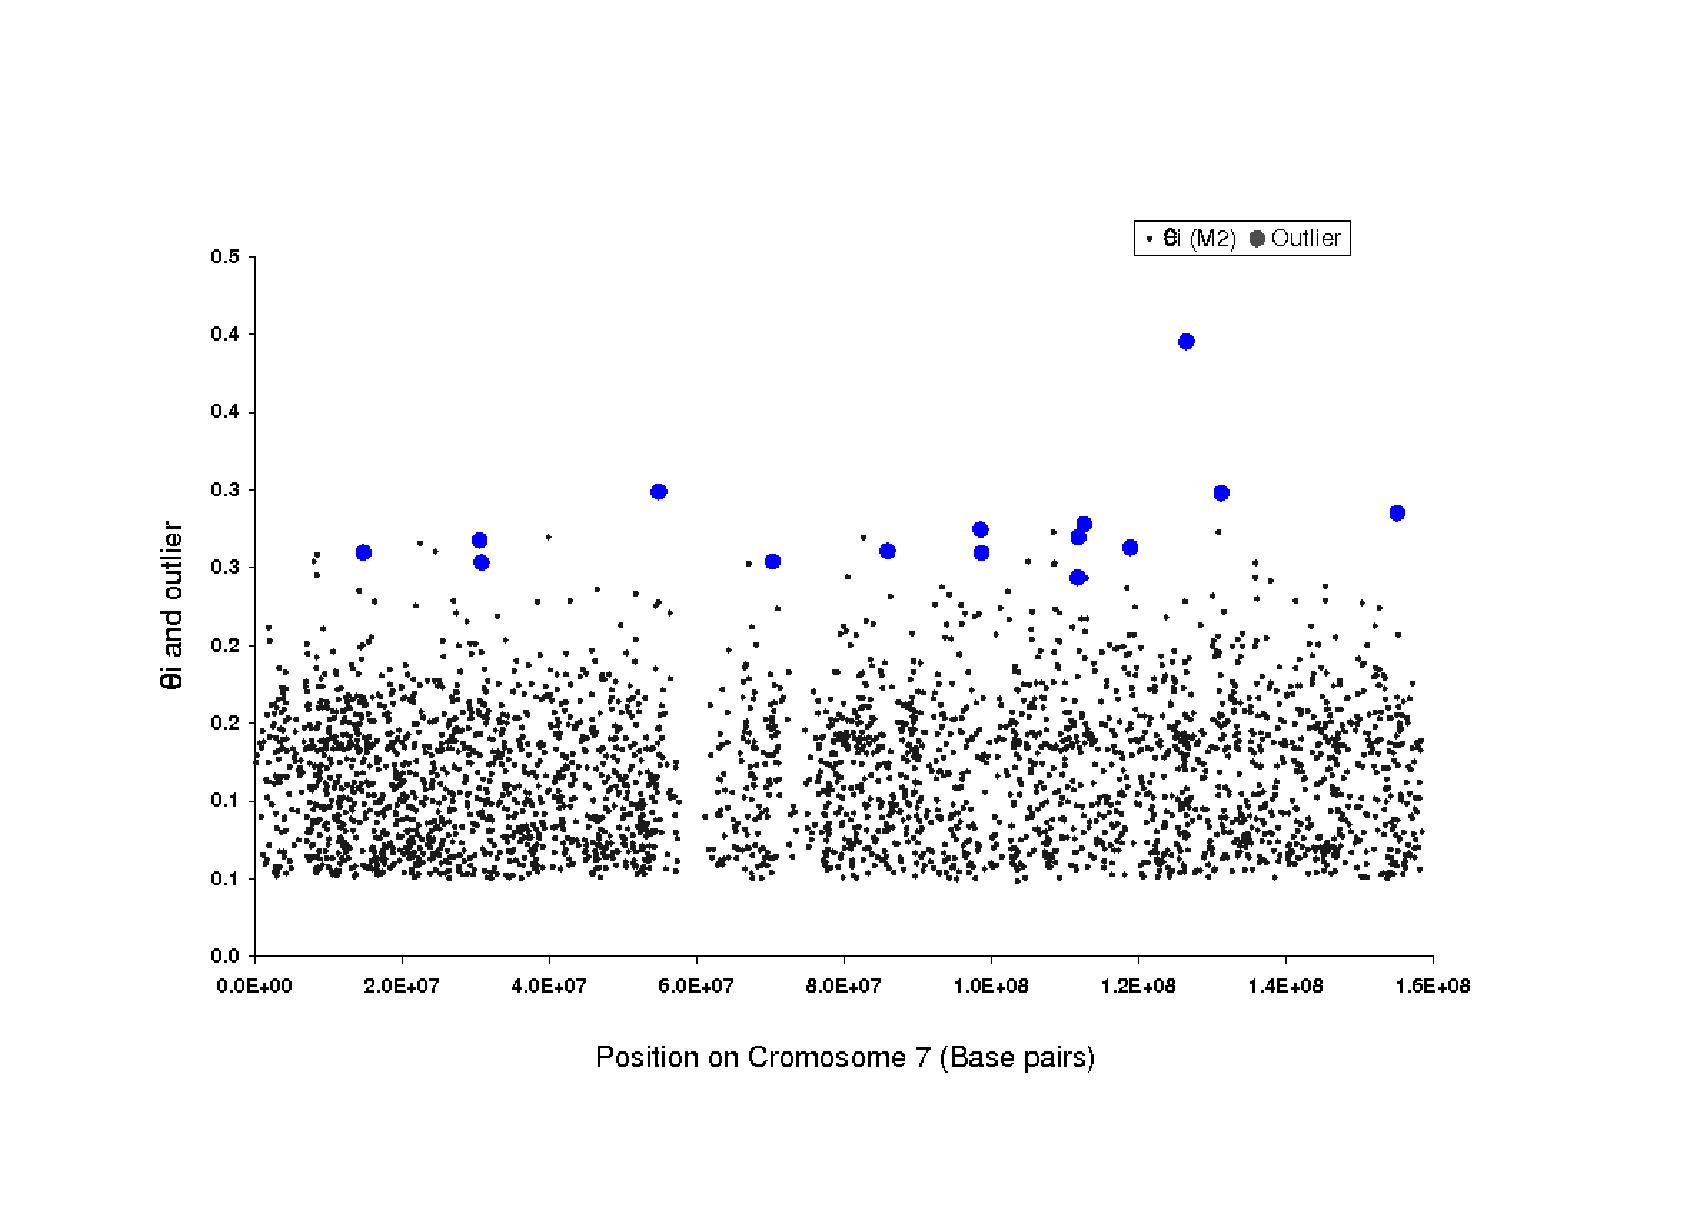
\includegraphics{outlier.eps}}
\end{center}
}

\myslide{
Average per nucleotide diversity
\begin{eqnarray*}
\pi &=& \sum x_ix_j\delta_{ij}/N \\
x_i &=& \mbox{frequency of haplotype $i$} \\
\delta_{ij} &=& \mbox{number of nucleotide differences between $i$ and
  $j$} \\
N &=& \mbox{length of haplotype sequence}
\end{eqnarray*}
}

\myslide{
Definition
\[
\theta = 4N_e\mu
\]
({\bf NOT} Weir \& Cockerham's $\theta$).
}

\myslide{
Under the infinite sites model of evolution
\begin{eqnarray*}
\E(\pi) &=& \theta \\
\E(k) &=& \theta\sum_i^{n-1} \frac{1}{i} \\
n &=& \mbox{number of haplotypes in the sample}
\end{eqnarray*}
\vfil
\begin{eqnarray*}
\hat \theta_\pi &=& \hat \pi \\
\hat \theta_k   &=& \frac{k}{\sum_i^{n-1}\frac{1}{i}} \\
\hat D &=& \hat\theta_\pi - \hat\theta_k 
\end{eqnarray*}
}

\myslide{
\begin{description}

\item[$\hat D = 0$:] We have no evidence for changes in population
  size or for any particular pattern of selection at the
  locus.

\item[$\hat D < 0$:] The population size may be increasing or we may
  have evidence for purifying selection at this locus.

\item[$\hat D > 0$:] The population may have suffered a recent
  bottleneck (or be decreaing) or we may have evidence for
  overdominant selection at this locus.

\end{description}
}

\end{document}

